%\documentclass[a4paper]{acmart}
\documentclass[sigplan,screen]{acmart}
\usepackage{booktabs}
\usepackage{listings}
\usepackage{amsmath}
\usepackage{microtype}
\settopmatter{printacmref=false}
\renewcommand\footnotetextcopyrightpermission[1]{}


%%%%%| FOR CUSTOMIZING ACM FORMATTING / HEADERS |%%%%%

% OPTION1: hide ACM headers completely...
% Hide ACM reference block and copyright footnote
%\settopmatter{printacmref=false}
%\renewcommand\footnotetextcopyrightpermission[1]{}
% Use plain page style (optional)
%\pagestyle{plain}

% OPTION2: override ACM headers with customizations...
\acmConference[Nuchwezi Research]{Proceedings on the TEA Language}{May '26}{K'la, UG}
\acmYear{2026}
%\acmISBN{}
%\acmDOI{}


% OPTION3: start document with review/submission-friendly class...
%\documentclass[manuscript,screen]{acmart}
% or for double-blind review
%\documentclass[manuscript,review,anonymous]{acmart}


%%%%% EXTRA/OTHER PREAMBLE

% preamble
\usepackage{xcolor}
\usepackage{listings}

% define a darker red
\definecolor{teaDarkRed}{HTML}{8B0000} % DarkRed

\lstdefinestyle{tea}{
  basicstyle=\ttfamily\small,
  frame=single,
  frameround=tttt,
  rulecolor=\color{black},
  captionpos=b,
  showstringspaces=false,
  % make '#' start a line comment and color it blue
  morecomment=[l][\color{blue}]{\#},
  commentstyle=\color{blue},
  % color every colon red (applies globally, including inside comments)
  %literate={:}{{\textcolor{teaDarkRed}{\textbf{:}}}}1  
  literate=
    {|}{{\textcolor{blue}{|}}}1
    {:}{{\textcolor{teaDarkRed}{\textbf{:}}}}1  
}

% for line-breaks in table cells
\usepackage{makecell}

% to include pdf pages
\usepackage{pdfpages}

% Define \invpi to flip the pi symbol and use it as a function
\newcommand{\invpi}[1]{\mathop{\rotatebox[origin=c]{180}{$\pi$}}#1}


\title{TEA: Transforming Executable Alphabet --- A Minimal Language Leveraging Sequence Transformer Chaining}

\author{Joseph W. Lutalo}
\affiliation{%
  \institution{Nuchwezi Research}
  \country{Uganda}}
\email{jwl@nuchwezi.com}

\begin{document}


% insert [front] cover --- could just be a PNG or PDF
%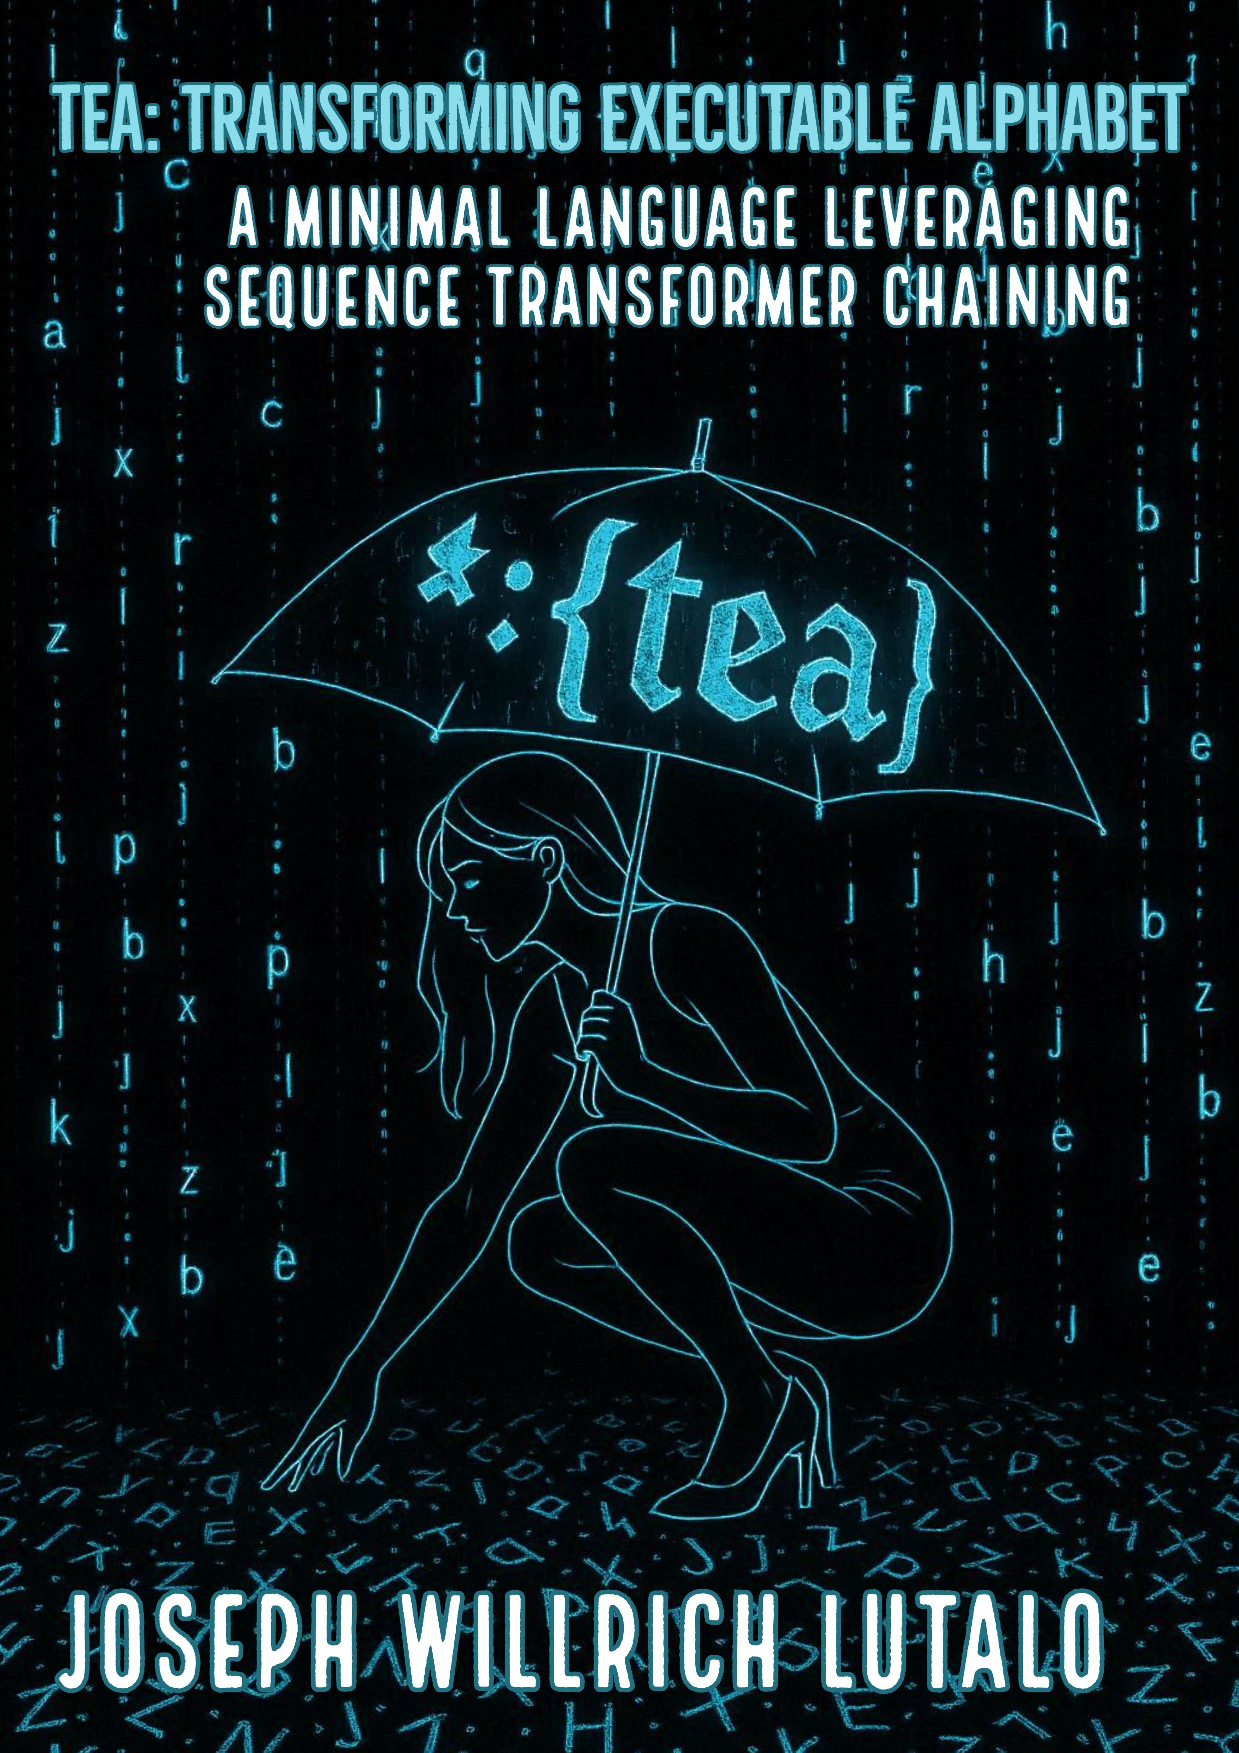
\includepdf[pages=1,fitpaper=true]{resources/pdf/frontcover.pdf}

% or explicitly stretch to page size
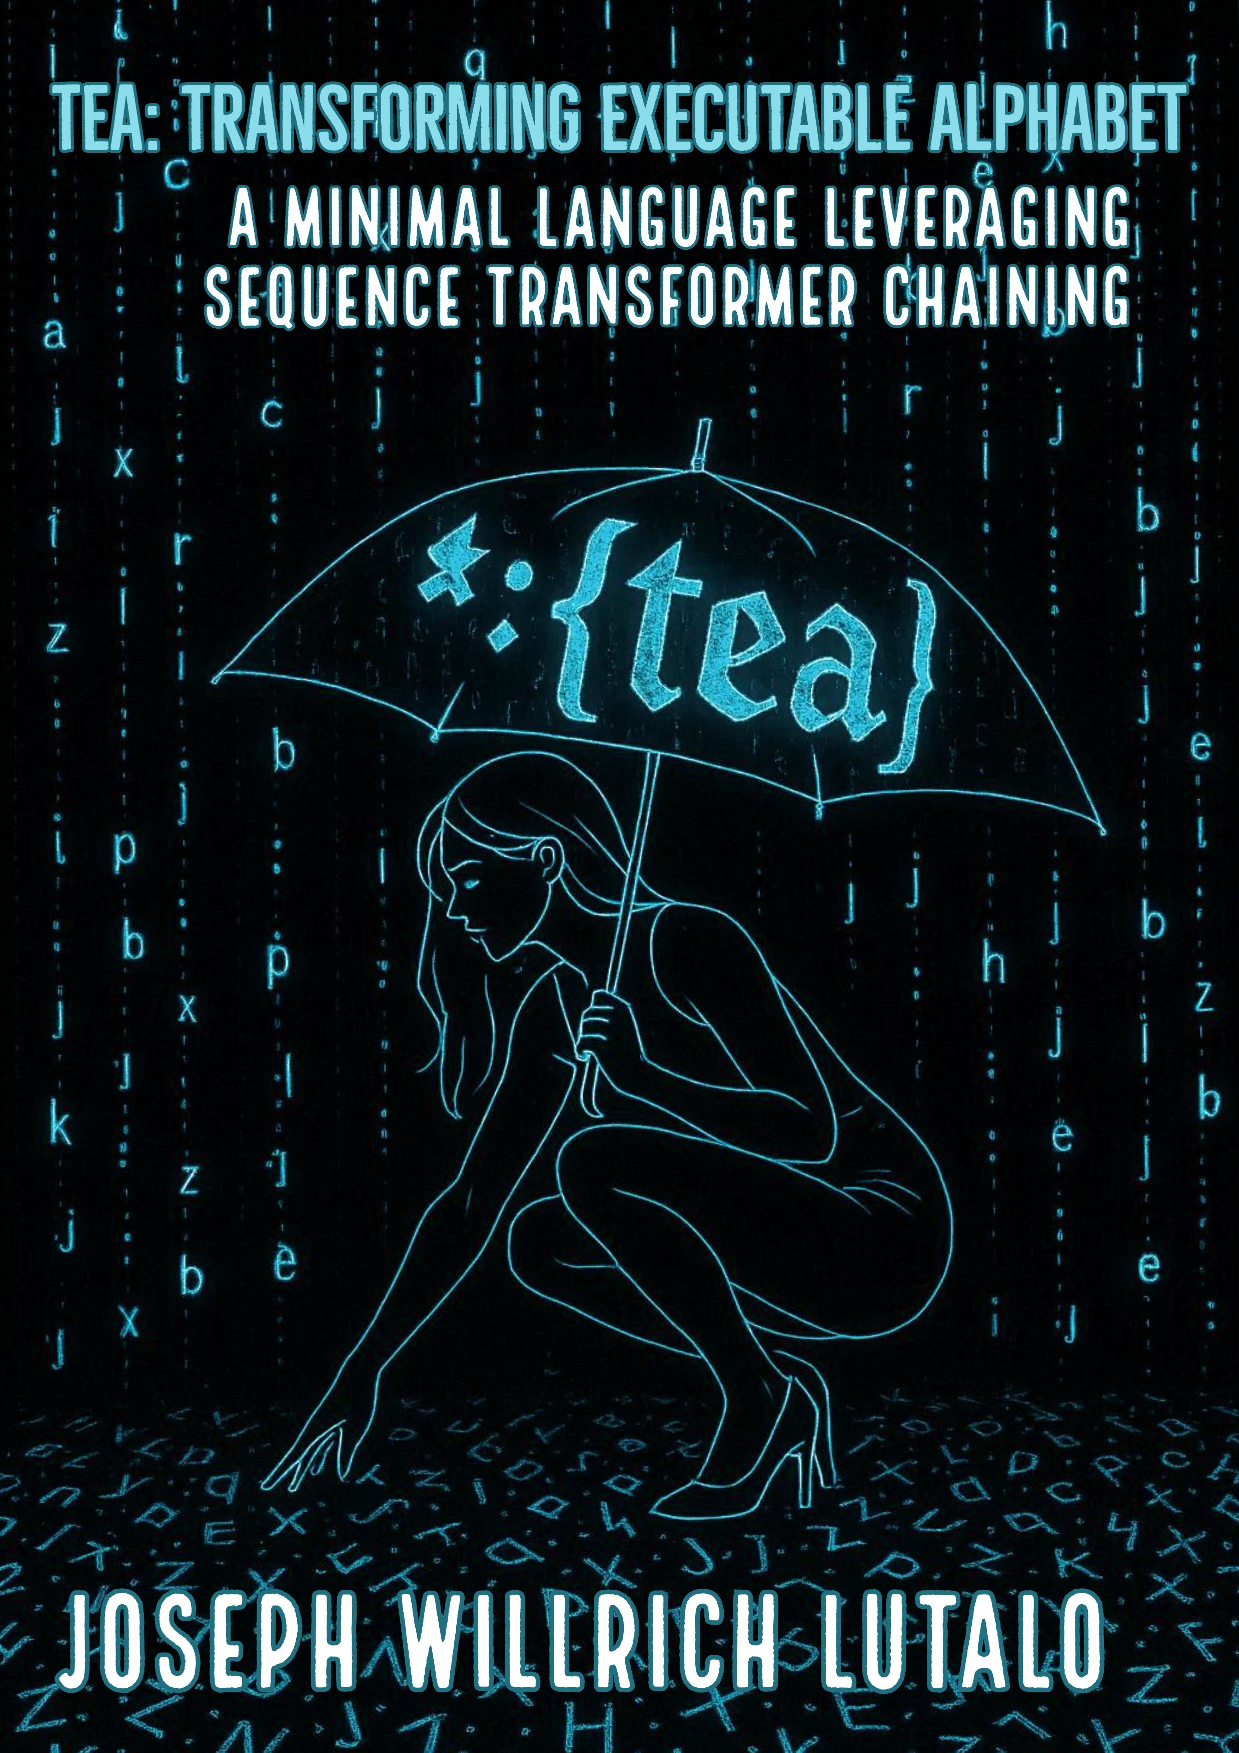
\includepdf[pages=1,
  width=\paperwidth,
  height=\paperheight,
  pagecommand={}]{resources/pdf/frontcover.pdf}


\begin{abstract}
We introduce the Transforming Executable Alphabet (TEA), a compact, general-purpose programming language designed around a \emph{sequence-transformer-chaining} paradigm and optimized for problem solving via text-processing. TEA's instruction set is intentionally minimal: the 26 Latin letters form the core commands, optionally qualified by a small set of symbols, producing a bounded global command space that enables concise programs, easy memorization, and powerful composition. TEA has been implemented as an interpreted language across platforms (using Python and JavaScript transpilers), supports embedded persistent storage, web client primitives, processing mathematics, and a rich text-processing standard library. We present the language design, formal semantics for instruction chaining, implementation strategies, representative applications (40+ sample programs), and an evaluation of its expressiveness, concision, and cross-platform performance. We conclude with a discussion of TEA's potential roles in education, low-resource mobile programming, and domain-specific sequence analysis.\\\\
\textbf{Keywords}: Language Engineering, Alphabet-based Languages, Language Semantics, Cross-Platform Development
\end{abstract}


\maketitle

\section{Introduction}
Modern software engineering increasingly demands languages that are compact, portable, and expressive for text and sequence manipulation \cite{lutalo2024software}. Designers of new languages are also encouraged to have users of the language in mind and especially to adopt a multidisciplinary approach to the design and evaluation of their new programming or software language \cite{coblenz2018interdisciplinary}. We present TEA (Transforming Executable Alphabet), a language designed from first principles to make sequence transformation concise, composable, and accessible on constrained devices.

\begin{quotation}``TEA is based on the idea of an instruction set whose core is just the 26 letters of the Latin Alphabet, and which we can qualify or decorate using a specific set of symbols known as command qualifiers, `.', `!', `*' and `@', so as to specify `qualified commands'.''\end{quotation}

TEA began as a mobile-first text-processing prototype in 2021 and has evolved into a cross-platform language with interpreters in JavaScript (web, mobile-web) and Python (elsewhere), a growing standard library, and a documented instruction set (the TEA TAZ \cite{Lutalo2024TEATAZ}). The language targets scenarios where compactness, offline capability, and text-centric transformations are primary concerns: mobile scripting, embedded text-processing, lightweight data engineering, and domain-specific sequence analysis among others.

\section{Design Goals and Rationale}
The TEA design is driven by the following goals:

\begin{itemize}
  \item \textbf{Minimal, memorable instruction set.} Use the 26 letters as primary command spaces to reduce cognitive load.
  \item \textbf{Composability.} Enable chaining of sequence transformers \cite{Lutalo2025_transformatics_thesis} to express complex pipelines succinctly.
  \item \textbf{Conciseness.} Allow programs to be expressed as single strings when needed (minified form).
  \item \textbf{Cross-platform portability.} Provide interpreters for web, mobile, desktop, and server environments.
  \item \textbf{Practical tooling.} Ship a standard library, sample programs, and a reference manual (TEA TAZ).
\end{itemize}

These goals reflect TEA's origin as a mobile-first language for low-resource environments and its subsequent maturation into a general-purpose text-processing language.

\section{Language Overview}
\subsection{Lexical and Syntactic Conventions}
A TEA instruction consists of a \emph{key letter} (A–Z or a–z), optionally qualified by one of the qualifier symbols \texttt{. ! * @}, followed by a colon \texttt{:} and zero or more parameters separated by colons. Instructions may be placed on separate lines (sanitized form), combined on a single line separated by vertical bars \texttt{|} (minified form), or mixed with comments beginning with \texttt{\#}.

\begin{lstlisting}[style=tea,caption=Minimal TEA Program Examples,label=LST1] 
i!:Hello World         # print `hello world'
n:1000:10              # RNG from [10,1000]
i!:{Name?}|i:|x:{Hi }  # name prompt + greet
\end{lstlisting}

\subsection{Command Space and Qualifiers}

% Command-space bound (qualifiers in fixed precedence)
\noindent Under the language's grammar rules \cite{Lutalo2024TEATAZ} we can form TEA commands using; one of 26 case‑insensitive letters, qualifiers drawn from the symbol set
$\{*,!,.,@\}$, each qualifier optional and used at most once, and when multiple qualifiers appear they must follow the fixed precedence order \texttt{* ! . @}---each qualifier is either present or absent, giving $2^{4}=16$ qualifier forms per letter (including the empty form). Multiplying by the 26 letters yields a total of


\[
26 \times 2^{4} = 416
\]


distinct TEA commands. This count includes the unqualified letter form and all combinations of one, two, three, or all four qualifiers written in the canonical order.

\begin{table}[ht]
  \centering
  \caption{Command-space combinatorics for TEA (fixed qualifier precedence).}
  \label{tab:tea-command-space}
  \begin{tabular}{@{}ll@{}}
    \hline
    \textbf{Attribute} & \textbf{Value} \\
    \hline
    Letters (case) & 26 (case‑insensitive) \\
    Qualifier set & \(\{*,!,.,@\}\) \\
    Qualifier rule & \makecell[l]{Optional; no repetition;\\fixed precedence \texttt{* ! . @}} \\
    Qualifier forms per letter & \(2^{4}=16\) \\
    Total distinct commands & \(\mathbf{416}\) \\
    \hline
  \end{tabular}
\end{table}


Also, note that each letter denotes a \emph{command space} (e.g., \texttt{i:} for I/O, \texttt{n:} for numeric utilities, \texttt{r:} for rewrite and math etc.). Qualifiers modify semantics (for example, \texttt{r.:EXPR} is for evaluating math expressions, while \texttt{r:PAT:SUB} is for text rewriting \cite{Lutalo2024TEATAZ}). However, despite the global maximum number of distinct qualified commands being bounded, and yet, in practice, not all of these are currently being utilized. Conventionally, unutilized or undefined TEA commands are labeled or considered \textbf{INERT} \cite{Lutalo2024TEATAZ}, generally have no effect in a TEA program, and might be flagged at runtime as part of dynamic program validation or debugging \cite{Lutalo2025debug}.

\section{Formal Semantics}
\label{sec:formal-semantics}

This section gives a concise, mathematically grounded semantics for TEA suitable for a SLE paper.  We combine the language definition excerpted from the TEA TAZ with a compact operational model based on \emph{sequence-transformer chaining} \cite{Lutalo2025_transformatics_thesis}. 

\subsection{Overview and notation}
We model TEA programs as ordered sequences of \emph{TEA instructions} (TIs).  Let \(\Sigma\) denote the set of TEA strings (UTF-8 text).  A TEA instruction \(t\) is a syntactic object formed from a \emph{key letter} \( \ell \in \mathcal{L} \) (where \(\mathcal{L}=\{a,\dots,z\}\) is case-insensitive) optionally followed by a qualifier pattern \(q\) drawn from the canonical qualifier order \(\mathcal{Q} = \langle *,!,.,@\rangle\) and zero or more colon-separated parameters.  A TEA program of length \(n\) is an ordered tuple


\[
\mathbb{T}^n = (t_1, t_2, \dots, t_n).
\]


We write \(I\) for an arbitrary sequence value (the \emph{TEA input/state}) and \(O\) for the program output/state.

\subsection{Sequence-transformer chaining (informal)}
Each instruction \(t_i\) denotes a \emph{transformer} \(T_{t_i}\), a (possibly partial) function from sequences to sequences:


\[
T_{t_i} : \Sigma^* \rightharpoonup \Sigma^*.
\]


Execution of a program \(\mathbb{T}^n\) on initial input \(I_0\) composes these transformers left-to-right to produce a final output \(O\):


\[
I_0 \xrightarrow{t_1} I_1 \xrightarrow{t_2} I_2 \cdots \xrightarrow{t_n} I_{n} = O,
\]


equivalently \(O = (T_{t_n}\circ \cdots \circ T_{t_2}\circ T_{t_1})(I_0)\).  This presentation follows the sequence-transformer chaining paradigm and aligns with the Transformatics perspective on ordered sequence processing \cite{Lutalo2025_transformatics_thesis}.

\subsection{Small-step operational semantics}
We present a small-step operational semantics that captures deterministic instruction evaluation and state threading.  A \emph{configuration} is a pair \((\mathbb{T}^n, I)\) where \(\mathbb{T}^n\) is the remaining instruction sequence and \(I\) the current state.  The one-step relation \(\longrightarrow\) is defined by the rule below:



\[
\frac{T_{t_1}(I) = I'}{(t_1, t_2, \dots, t_n; I) \longrightarrow (t_2, \dots, t_n; I')}
\qquad\text{(STEP)}
\]



If \(T_{t_1}\) is undefined on \(I\) (partial transformer failure or an \textit{inert} TI), the configuration is stuck; practical interpreters may perhaps raise an error or perform a recovery action (logging, fallback transformer, etc.). In current implementations though, we generally merely skip or ignore specifically inert TI, passing on $I_{i-1}$ to $T_{t_{i+1}}$ when $T_{t_{i}}$ failed or was inert. Some commands though, also merely set $I' = ``" = I_{i+1}$ in such a case; set current transformer output as the \texttt{EMPTY SPACE} upon encountering a runtime error \cite{Lutalo2024TEATAZ}.  Multi-step execution is the reflexive transitive closure \(\longrightarrow^{*}\).  Termination with output \(O\) is:



\[
(t_1,\dots,t_n; I_0) \longrightarrow^{*} (\; ; O) \quad\text{iff}\quad O = (T_{t_n}\circ\cdots\circ T_{t_1})(I_0).
\]



\subsection{Big-step semantics (evaluation judgment)}
For many proofs and reasoning tasks a big-step (evaluation) judgment is convenient.  We write


\[
\langle \mathbb{T}^n, I \rangle \Downarrow O
\]


to mean that program \(\mathbb{T}^n\) evaluates on input \(I\) to produce \(O\).  The big-step rules are:



\[
\frac{}{\langle \; , I \rangle \Downarrow I} \qquad\text{(E-Empty)}
\]

and

\[
\frac{\langle (t_2,\dots,t_n),\; I' \rangle \Downarrow O \quad T_{t_1}(I)=I'}{\langle (t_1,t_2,\dots,t_n),\; I \rangle \Downarrow O} \qquad\text{(E-Step)}
\]



These rules are equivalent to the small-step semantics under standard determinism assumptions for the transformers.

\subsection{Transformer classification and side effects}
Transformers fall into two broad classes:

\begin{itemize}
  \item \textbf{Pure transformers:} \(T\) depends only on its input sequence and returns a new sequence; these are total or partial pure functions \( \Sigma^* \rightharpoonup \Sigma^* \).
  \item \textbf{Effectful transformers:} \(T\) may perform I/O, persistent storage updates, or network actions.  We model effectful transformers as functions that thread an explicit \emph{world} or effect state \(W\): \(T : (\Sigma^*, W) \rightharpoonup (\Sigma^*, W)\).  For the formal core we separate pure evaluation from effect handling; the interpreter semantics composes effectful steps in a deterministic scheduling policy.
\end{itemize}

\subsection{Properties}
\paragraph{Determinism.} If every transformer \(T_{t}\) is deterministic on its domain and the interpreter enforces a fixed evaluation order, then program evaluation is deterministic: for given \(\mathbb{T}^n\) and \(I_0\) there is at most one \(O\) such that \(\langle \mathbb{T}^n, I_0\rangle \Downarrow O\).

\paragraph{Compositionality.} The semantics is compositional: the meaning of a program is the composition of the meanings of its instructions.  Formally, if \(\mathbb{T}^n = \mathbb{T}^k \mathbin{+\!\!+} \mathbb{T}^{n-k}\) (concatenation), then for all \(I\),


\[
\langle \mathbb{T}^n, I \rangle \Downarrow O \quad\Longleftrightarrow\quad
\exists I'.\; \langle \mathbb{T}^k, I \rangle \Downarrow I' \ \wedge\ \langle \mathbb{T}^{n-k}, I' \rangle \Downarrow O.
\]



\paragraph{Reasoning about partiality and errors.} Because many transformers are partial (e.g., parsing failures, network timeouts), program correctness proofs must account for stuck configurations or effectful recovery rules.  We recommend using a totalization strategy (option types or explicit error values) in formal proofs and in critical interpreter components.

\subsection{Relation to Transformatics}
The TEA semantics directly implements the Transformatics view of ordered sequence processing: TEA instructions are first-class sequence transformers and program execution is their ordered composition. Also, for any sequence of TEA instructions specifying a particular program for some purpose, the entire sequence of instructions is considered a \textbf{higher-order sequence transformer}.  This alignment provides a principled basis for reasoning about TEA programs using the mathematical tools developed in Transformatics \cite{Lutalo2025_transformatics_thesis}.

\subsection{Implementation notes}
The reference interpreters (Python, JavaScript) implement the above semantics with a lexer/parser that normalizes sanitized, minified, and mixed forms into an internal instruction list that is essentially of sanitized form, an execution engine that applies transformers in left-to-right order, and an effect manager that sequences I/O and persistent storage operations deterministically.  The repository and language manual provide the concrete transformer definitions and examples used in the semantics above \cite{cli_tttt,Lutalo2024TEATAZ}.

% End of Formal Semantics section


\section{Implementation}
\subsection{Reference Interpreters}
Reference interpreters exist in Python (command-line) and JavaScript (web). The interpreters implement a modular pipeline:
\begin{enumerate}
  \item \textbf{Lexing/Parsing:} Tokenize instructions, qualifiers, parameters, and comments.
  \item \textbf{Normalization:} Convert sanitized/minified/mixed forms into an internal instruction list.
  \item \textbf{Execution Engine:} Evaluate transformers sequentially, manage state, I/O, and persistent storage.
  \item \textbf{Standard Library:} Implementations for each command space (A–Z) with documented semantics.
\end{enumerate}

The TEA GitHub repository hosts the reference implementations, sample programs, and documentation, however, interested users and students might immediately access a live TEA language environment (akin to a \textit{language workbench} or integrated development environment (IDE)) via: \url{https://tea.nuchwezi.com} 

\subsection{Persistent Storage and Web Primitives}

TEA includes a lightweight embedded database (``TEA Database" --- essentially a no-SQL key-value storage) for portable scripts, but also primitives for HTTP GET/POST with allowance for setting custom headers and advanced content and request parameter processing. These features enable TEA programs to act as tiny, but robust web clients, API glue, and offline-capable utilities with guaranteed device-specific persistence.

\section{Tooling, Ecosystem, and Examples}
TEA ships with:
\begin{itemize}
  \item \textbf{TEA TAZ:} The language manual and command-space specification \cite{Lutalo2024TEATAZ}.
  \item \textbf{40+ sample programs\footnote{Readily accessible, usable via \textbf{TEA WEB IDE} but also via the \textit{offline-capable} \textbf{TEA MOBILE IDE} \url{https://bit.ly/teamobile_apks}}:} Examples spanning calculators, data engineering, chatbots, games, cryptography, and a proof-of-concept TEA OS.
    \item \textbf{Command-line package (TTTT):} A Debian package\footnote{Quick, secure installation [on your server] via:\\ \texttt{curl -Ls https://bit.ly/installtea | bash}} that adds the TEA interpreter as well as some TEA utilities (AMC, ZHA and Lexicon) to any Linux-compartible system for both developers and normal users to leverage TEA.
  \item \textbf{Mobile app (mobile TTTT):} A compact TEA IDE for Android enabling offline development and running or sharing TEA programs and their outputs.
\end{itemize}

Minimal representative examples include:
\begin{itemize}
  \item \textbf{Hello World:} \texttt{i!:Hello World}
  \item \textbf{Generate Random IP Address:} \texttt{n!:256:0:4:.}
  \item \textbf{Process Mathematics:} \texttt{r.:{1/2*(1 + 5**(2**(-1)))}}
  \item \textbf{Shuffle List of Words:} \texttt{a:\{one two three go\}}
\end{itemize}

And for a more involved minimal example, consider the following TEA program that fetches, preprocesses and presents \textbf{random jokes} from some WEB API:


\begin{lstlisting}[style=tea,caption=EDUTAINMENT: Random Jokes v2.1,label=LST2]                    
                   
i!:https://
x!:utility.nuchwezi.com
x!:/random/jokes
w:
h!:,
k:{setup|punchline}
h!:{:}
k!:{setup|punchline}
d.::.
r!:.\n:_
d:.$
h!:_
d:_
\end{lstlisting}


It essentially triggers an HTTP GET request, parses and cleans the returned JSON payload, and then produces neat outputs such as \textit{``Why are skeletons so calm?
Because nothing gets under their skin."}

\section{Evaluation}
We evaluate TEA along three axes: \textbf{concision}, \textbf{expressiveness}, and \textbf{performance}.

\subsection{Concision}

TEA programs are often extremely short in character count. The Hello World example demonstrates minimal syntactic overhead, and if we were to measure program length (characters) for a set of canonical tasks and compare TEA to both classical (COBOL, LISP, C, Sed,...) and modern languages (Python, JavaScript, Go, Ruby,...), one would generally find that, by metrics and cases such as the 8 covered in the DNAP SOE language evaluation suite \cite{lutalo2023dnapsoe}, TEA would arguably outshine most of the competition. Consulting \textbf{\hyperref[LST3]{Listing \ref{LST3}}} should help drive this home.

\subsection{Expressiveness}
Using the sequence-transformer chaining model, TEA expresses many text-processing pipelines succinctly. With the extra advantage that its instruction set almost exhaustively caters for most text-processing oriented problem solving via a suite of orthogonal transformers for arbitrary general problems, that one can then readily take any or most kinds of computational problems and model it using sequence transformers and their chaining, and thus readily harness TEA for realizing their specified solution. In this regard, TEA is arguably a very dependable and lightweight prototyping platform for personal, business, academic and scientific computation problems. In the TAZ, we present numerous case studies to demonstrate this power: a text-based adventure game (``Boobs `N' Traps'') \cite{lutalo_2025_rpg}, a q-AGI chatbot prototype (ZHA) \cite{lutalo2025unraveling}, and a DNA/RNA sequence analysis pipeline (from the Applying Transformatics in Genetics work) \cite{lutalo_2025_trans_genetics}, the LUMTAUTO bi-directional encryption \cite{lutalo_2025_grimlumtauto} and more as one shall find in \cite{Lutalo2024TEATAZ}. These case studies show TEA's ability to encode domain logic compactly.

\subsubsection{TEA Instruction Set Expressiveness}

Briefly, we shall look at why the minimal instruction design used in this language was chosen; ease of recall via a mnemonic naming of the inbuilt ``instruction library", the desire to encourage meaningful program composability via use of orthogonal instructions and of course, leveraging the sequence transformer chaining paradigm. With \textbf{\hyperref[tab:tea-az-minimal]{Table \ref{tab:tea-az-minimal}}}, we present the \textbf{26 command spaces} that define the TEA language instruction set; A: to Z: and their orthogonal purpose for authoritative reference purposes.

\begin{table*}[ht]
  \centering
  \small
  \caption{TEA instruction set summary (A--Z): primitive, command space name, and its concise purpose within the language.}
  \label{tab:tea-az-minimal}
  \begin{tabular}{@{}p{0.08\textwidth} p{0.24\textwidth} p{0.60\textwidth}@{}}
    \toprule
    \textbf{Primitive} & \textbf{Name} & \textbf{Purpose (distilled from TEA TAZ)} \\
    \midrule
    A: & \texttt{Anagrammatize} & Produce anagrams or shuffle symbols/lists for randomized reorderings. \\
    B: & \texttt{Basify} & Extract a lexical base or canonical symbol sequence for keys and comparisons. \\
    C: & \texttt{Clear} & Reset working memory or named vaults; initialize storage to empty. \\
    D: & \texttt{Delete} & Remove matched content or filter out unwanted patterns/whitespace. \\
    E: & \texttt{Evaluate} & Treat stored text as TEA code; execute or securely evaluate generated code. \\
    F: & \texttt{Fork} & Perform conditional branching via pattern tests; enable logic about program state. \\
    G: & \texttt{Glue} & Concatenate or bind tokens; remove whitespace/punctuation to form strings. \\
    H: & \texttt{Hew} & Split or explode text by pattern; introduce line breaks and lossless splits. \\
    I: & \texttt{Interact} & Set or prompt the Active Input (AI); force or conditionally assign AI. \\
    J: & \texttt{Jump} & Static program jumps and label-based control flow (unconditional loops). \\
    K: & \texttt{Keep} & Line-level filtering: retain only lines or segments matching user patterns. \\
    L: & \texttt{Label} & Define named code blocks / labels to enable conditional branching and encapsulation. \\
    M: & \texttt{Mirror} & Reverse or reflect text (characters, words, or multi-line inversion). \\
    N: & \texttt{Number} & Produce numeric/entropy values; support randomness and stochastic modeling. \\
    O: & \texttt{Order} & Sort tokens or sequences (lexical, numeric, or custom ordering). \\
    P: & \texttt{Permutate} & Generate permutations or structured/random strings from a given alphabet. \\
    Q: & \texttt{Quit} & Terminate execution (conditionally or unconditionally); support cut‑points. \\
    R: & \texttt{Replace/Rewrite} & Perform pattern-based substitution and general rewrite transformations. \\
    S: & \texttt{Salt} & Randomly inject or delete characters/spaces or perturb text for variation. \\
    T: & \texttt{Transform} & Apply formatting/structural transforms (trim, align, other string transforms). \\
    U: & \texttt{Uniquefy} & Extract unique items and frequency-based projections (modal statistics). \\
    V: & \texttt{Vault} & Named storage facility: read/write persistent or ephemeral data (variables). \\
    W: & \texttt{Webify} & Network I/O: HTTP GET/POST and interactions with web APIs or remote endpoints. \\
    X: & \texttt{Xenograft} & Affix prefixes/suffixes, replicate or reduce text to build parametric strings. \\
    Y: & \texttt{Yank} & Read memory/vaults and access stored or initial input values. \\
    Z: & \texttt{Zap} & External/effectful operations: non‑TEA evaluation, case transforms, introspection. \\
    \bottomrule
  \end{tabular}
\end{table*}


As one shall find when consulting the definitive and authoritative formal reference concerning the language's instruction set and each command space semantics, usage notes, examples and quirks --- essentially the TEA TAZ: \cite{Lutalo2024TEATAZ} --- for any particular TEA primitive, such as \texttt{V:} (\textbf{VAULT}), one finds well documented, an exhaustive breakdown of what each of the \textbf{active} (as opposed to \textit{inert}) command signatures are which are currently supported for the primitive. We see an example illustrated succinctly as in \textbf{\hyperref[tab:tea-v-semantics]{Table \ref{tab:tea-v-semantics}}}. Such should help the [amateur] TEA programmer understand how to leverage or interpret the particular commands supported in that TEA primitive's arsenal so as to fulfill one or more of the purposes laid down for that command space\footnote{In TEA, unlike many other languages perhaps, the rule of thumb is: \textbf{Read the M*F\#@ Manual First!} As well as when in doubt. Otherwise, despite the apparent simplicity of the language's syntax, you'll without doubt readily get lost, throw a tantrum or pull out your hair... utterly confused; gazing at a TEA program written by someone else --- such as the infamous \textbf{TEA OS}: \url{http://bit.ly/run_teaos} --- or perhaps trying to debug a thorny case in your own TEA codes, and then go wondering (or even wandering)... with possibly the arcane ancient wyzard daemon bickering-on at the back of your mind... \textit{\texttt{Proco Proco! Est!} Abandon all hope, ye thus entering here! Abandon all hope!} And well, of course, the smarter, seasoned engineer or hacker might sometimes decide to abandon hope looking for a solution via reading the [sometimes out-of-sync] manuals or TEA documentation, and instead directly go study the actual TEA transpiler source \cite{cli_tttt} --- it's a commendable and undaunting route given how clean and well maintained that code generally is.}. 


\begin{table}[ht]
  \centering
  \small
  \caption{Example Reference Semantics for the TEA \texttt{V:} (vault) instruction family.}
  \label{tab:tea-v-semantics}
  \begin{tabular}{@{}p{0.3\linewidth} p{0.6\linewidth}@{}}
    \toprule
    \textbf{Signature} & \textbf{Semantics (in summary)} \\
    \midrule
    \texttt{v:} & Store the Active Input (AI) into the default (unnamed) vault; if AI is unset, store the empty string. Returns AI. \\
    \hline
    \texttt{v:vNAME} & Store AI into named vault \texttt{vNAME}; returns AI. \\
     \hline
    \texttt{v:vNAME:VALUE} & Store literal \texttt{VALUE}(instead of AI) into vault \texttt{vNAME}; returns AI. \\
     \hline
    \texttt{v!:} & Return the length of the value in the default vault. \\
     \hline
    \texttt{v!:STR} & Return the length of literal string \texttt{STR}. \\
     \hline
    \texttt{v*:vNAME} & Force‑write AI into vault \texttt{vNAME}, overriding existing content; returns AI. \\
     \hline
    \texttt{v*:vNAME:VALUE} & Force‑write literal \texttt{VALUE} into vault \texttt{vNAME}; returns AI. \\
     \hline
    \texttt{v*!:vNAME} & Return the length of the value stored in vault \texttt{vNAME} (no name = same as \texttt{v!:}). \\
     \hline
    \texttt{v@:vNAME} & Persist AI under key \texttt{vNAME} in the TEA database (persistent vault); returns AI. \\
     \hline
    \texttt{v@:vNAME:VALUE} & Persist literal \texttt{VALUE} under key \texttt{vNAME} in the TEA database; returns AI. \\
     \hline
    \texttt{v!@:vNAME} & Return the length of the value stored in the TEA database under key \texttt{vNAME}. \\
    \bottomrule
  \end{tabular}
\end{table}

 So, for example, based on the semantics laid down in \textbf{\hyperref[tab:tea-v-semantics]{Table \ref{tab:tea-v-semantics}}}, we can then read and make sense of the following TEA program...
 


% in document
\begin{lstlisting}[style=tea,caption=Basic 8-character Password Generator, label=LST3]
####[ Basic Password Generator ]####
####################################

#---[ START ]
#given some initial/external seed...
I:{SOMEVALUE} #if none, then use our own seed
G!:|A!: #glue and anagrammatize seed
V:vSRC|V*!:vSRC #store it + return its size
Q:^0$ #quit if seed was empty; returns 0

#---[ PROCESS ]
V:vPWD:{} #init password with empty string
L:lTEST #init named code-block; jump-to point
V*!:vPWD #get current length of password
#lPRODUCE if != 8chars long else goto lRETURN
F!:^8$:lPRODUCE:lRETURN 
L:lPRODUCE #another labeled-block starts here
Y:vSRC #fetch the seed
A!:|D!:^. #shuffle seed + pick only 1st char
V:vCHOSEN #store picked letter in a vault
G*:{}:vPWD:vCHOSEN #glue it with current pwd
V:vPWD | V*!:vPWD #store as new pwd, rtn len
J:lTEST #[re]jump to password length test

#---[ FINISH ]
L:lRETURN | Y:vPWD #return final password
\end{lstlisting}



\subsection{Performance}

Though detailed and rigorous benchmarking tests and data wont be presented here, preliminary informal benchmarks comparing the two Python and JavaScript-powered TEA interpreters on representative tasks has been conducted. Such tests spanned; string transformation throughput (such as in the \textit{Ghost Messages protocol} encoding and decoding); numeric workloads (such as in the \textit{Fibonacci Sequence generation} tasks); HTTP client tasks. Results indicate how these interpreters are competitive and impressively performant on tasks one might have utilized their host languages for. Of course, the language is still under active development and fine-tuning, and thus further optimization as well as authoritative quantitative evaluations are future work.

\section{Case Studies}
\subsection{Text Adventure: Boobs `N' Traps}


\begin{figure}[ht]
  \begin{center}
   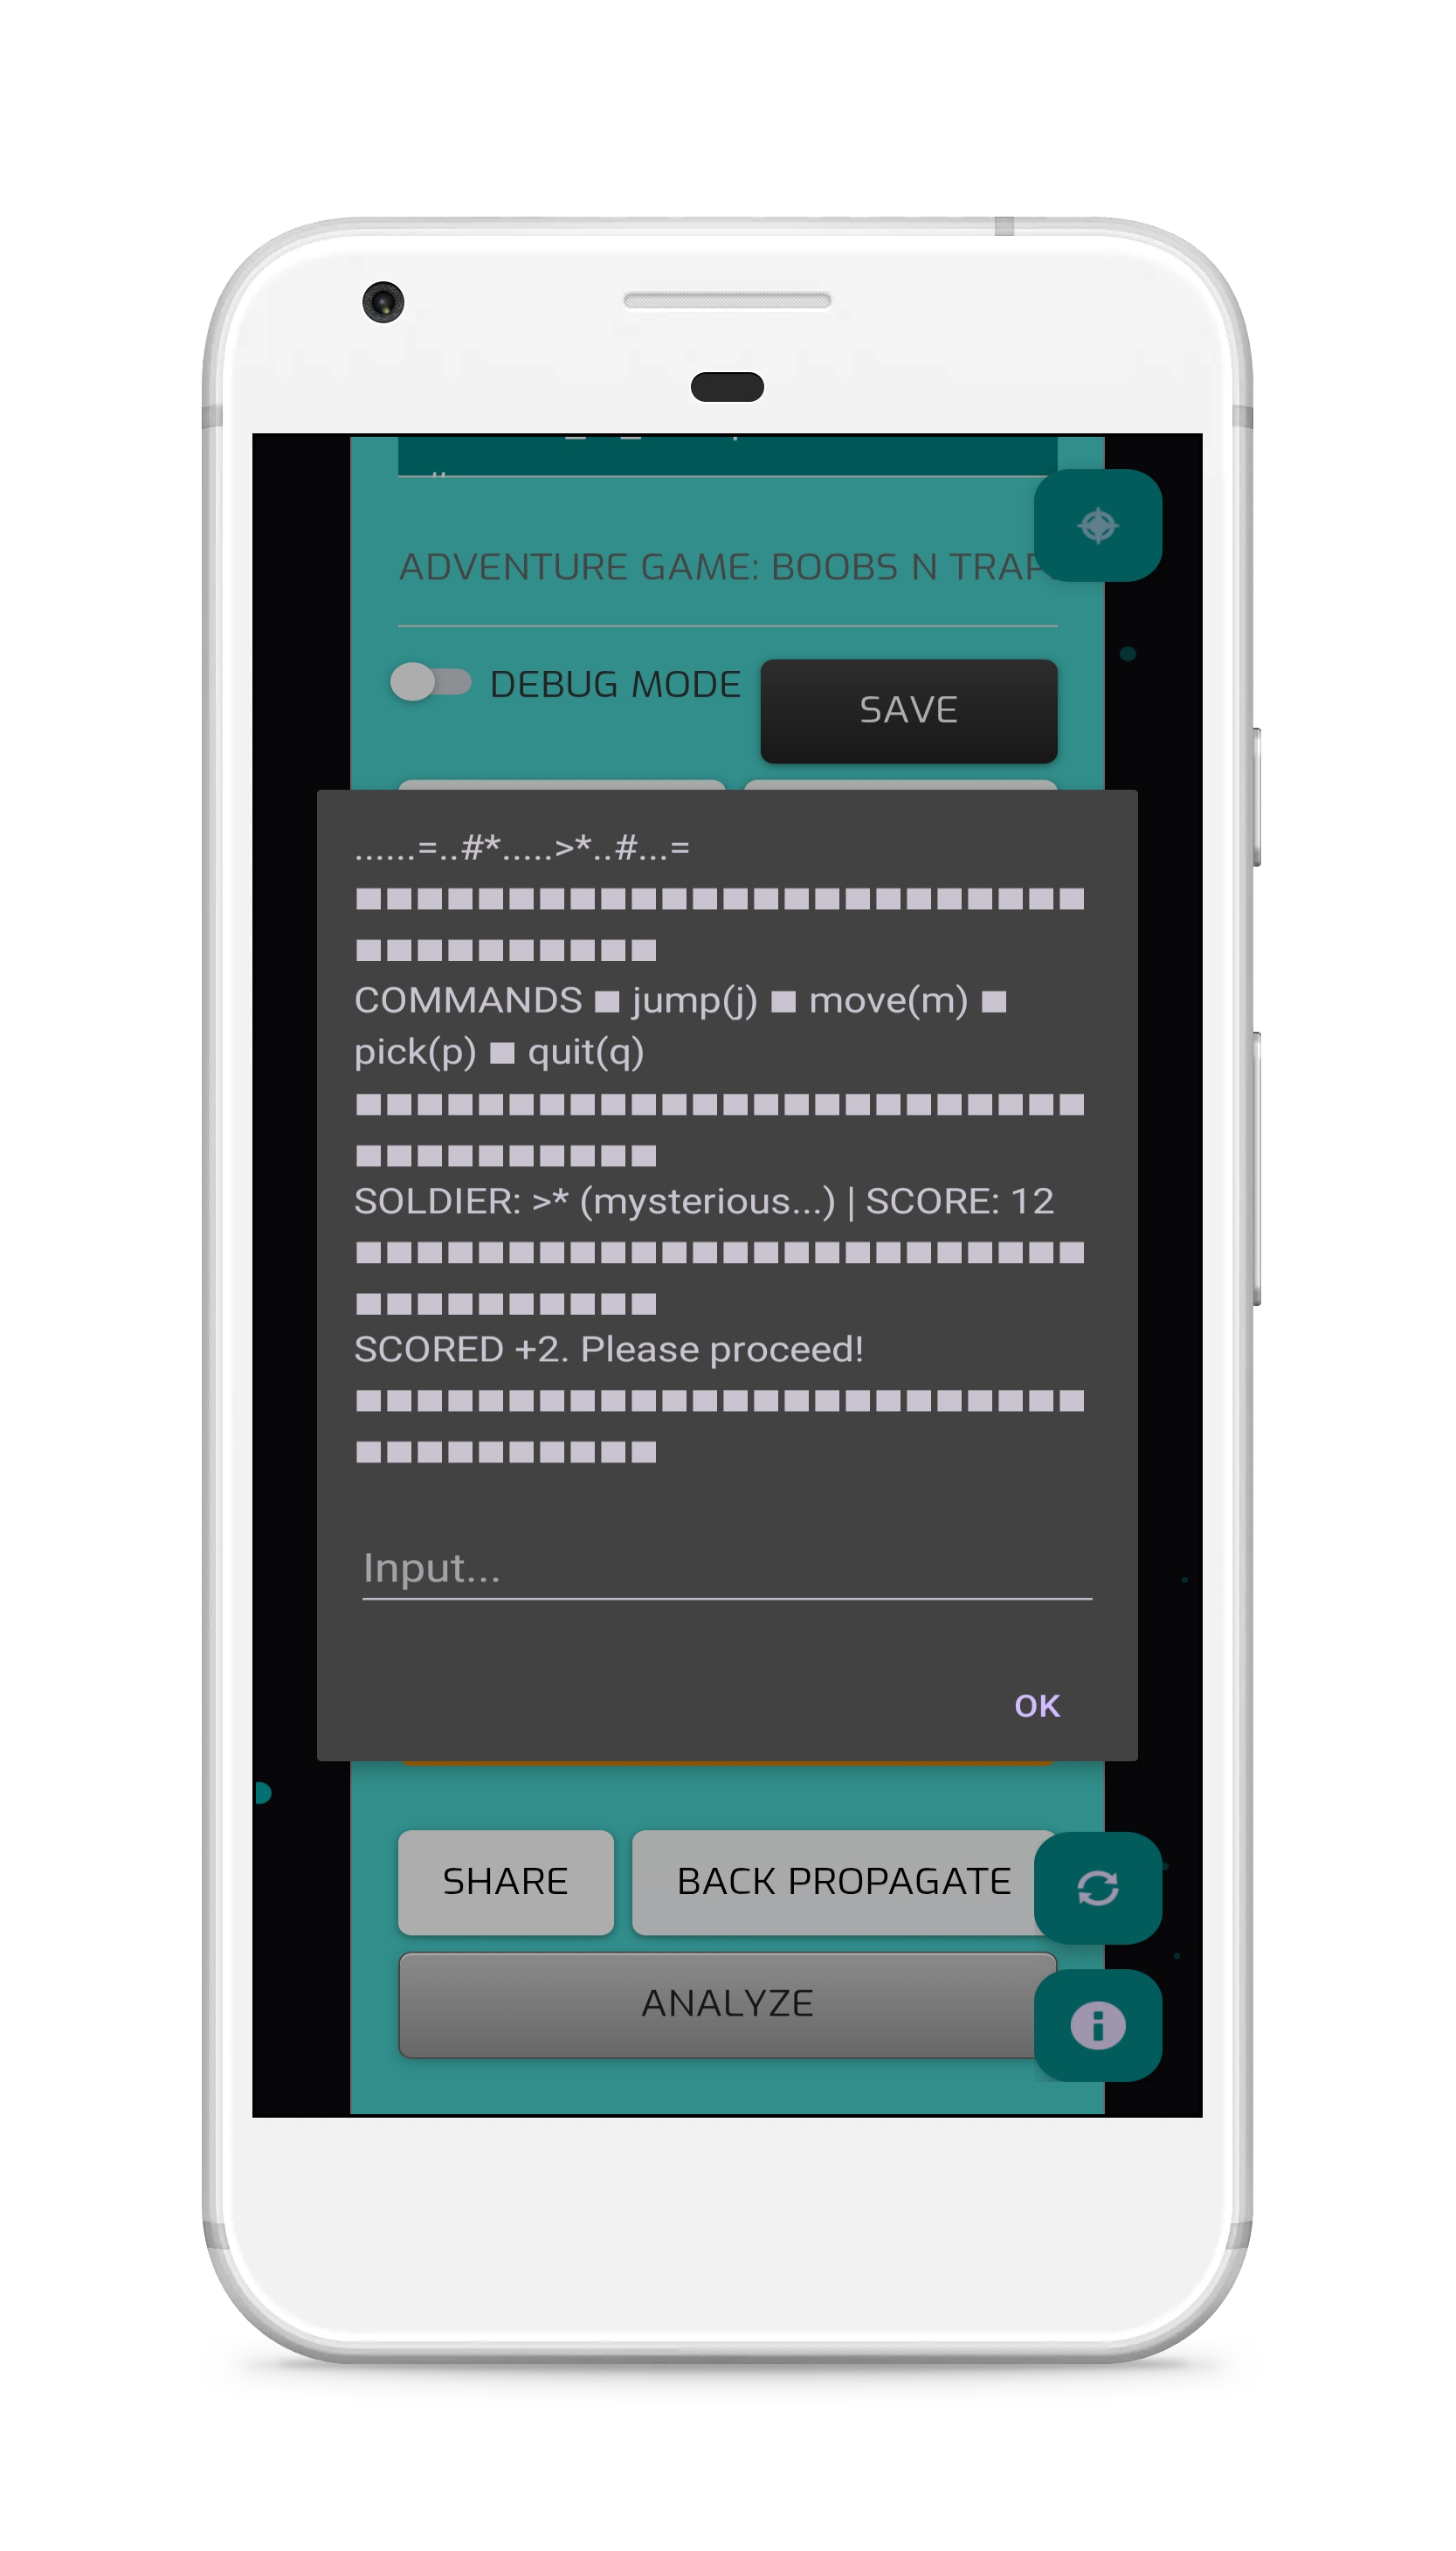
\includegraphics[width=0.4\textwidth]{resources/images/boobsntraps.png}\\
   \caption{BOOBS N TRAPS game session screen}
  \label{FIGBNT}
  \end{center}
\end{figure}


Inspired by classic command-line text-adventure RPG game, \textbf{NetHack}, this game demonstrates creative multi-strategy and reward logic, a minimal UI that is performant on any device, robust state-machine encoding, command-driven progress and input-command parsing and processing. It is among the best examples of what could be accomplished in pure TEA programming and the associated game state machine and design notes are documented as found in \cite{lutalo_2025_rpg}. \textbf{\hyperref[FIGBNT]{Figure \ref{FIGBNT}}} demonstrates what a typical game session feels and looks like on mobile.



\subsection{Sequence Analysis and Transformatics}

TEA has been applied to sequence analysis workflows in genetics; the language's sequence transformer chaining maps naturally to common bioinformatics pipelines as demonstrated in both \cite{lutalo_2026_19995017} and \cite{lutalo_2025_trans_genetics}. In particular, we find that TEA could be leveraged for problems such as:

\begin{enumerate}
\item \textbf{Genetic Fingerprinting} --- determining what the quantifiable similarities and differences between two or more genetic code sequences might be based on computing their modal sequences, sequence characteristics and for clusters or corpora, their population characteristic, etc.
\item \textbf{Genome Expression} --- by leveraging sequence transforms such as the mapping of DNA or RNA to decimal sequences and vice versa (such as in the proposed \textbf{Lu-Genome Expression System} \cite{lutalo_2025_trans_genetics}), one can readily apply algebraic and visual-spatial rendering techniques to the analysis and comparison of genetic sequences.
\end{enumerate}

\subsection{Chatbot and q-AGI Prototyping}

ZHA is short for ``Zee Hacker Assistant", a special chatbot with an interaction mode reminiscent of how hackers on IRC might ideally chat. Originally based off of earlier TEA-powered chatbots such as PA and TEAPA \cite{lutalo2025unraveling}, but also inspired by earlier work in human support via chatbots such as with the VOSAC \cite{lutalo2024vosa} Question-Answer Knowledge-Base driven voice chatbot, ZHA demonstrates TEA's suitability for rapid prototyping of conversational agents using compact transformation pipelines, offline-reliability via meaningful auto-generated content as well as the potential to leverage TEA's embedded persistence and neat text document generation capabilities.


\begin{figure}[ht]
  \begin{center}
   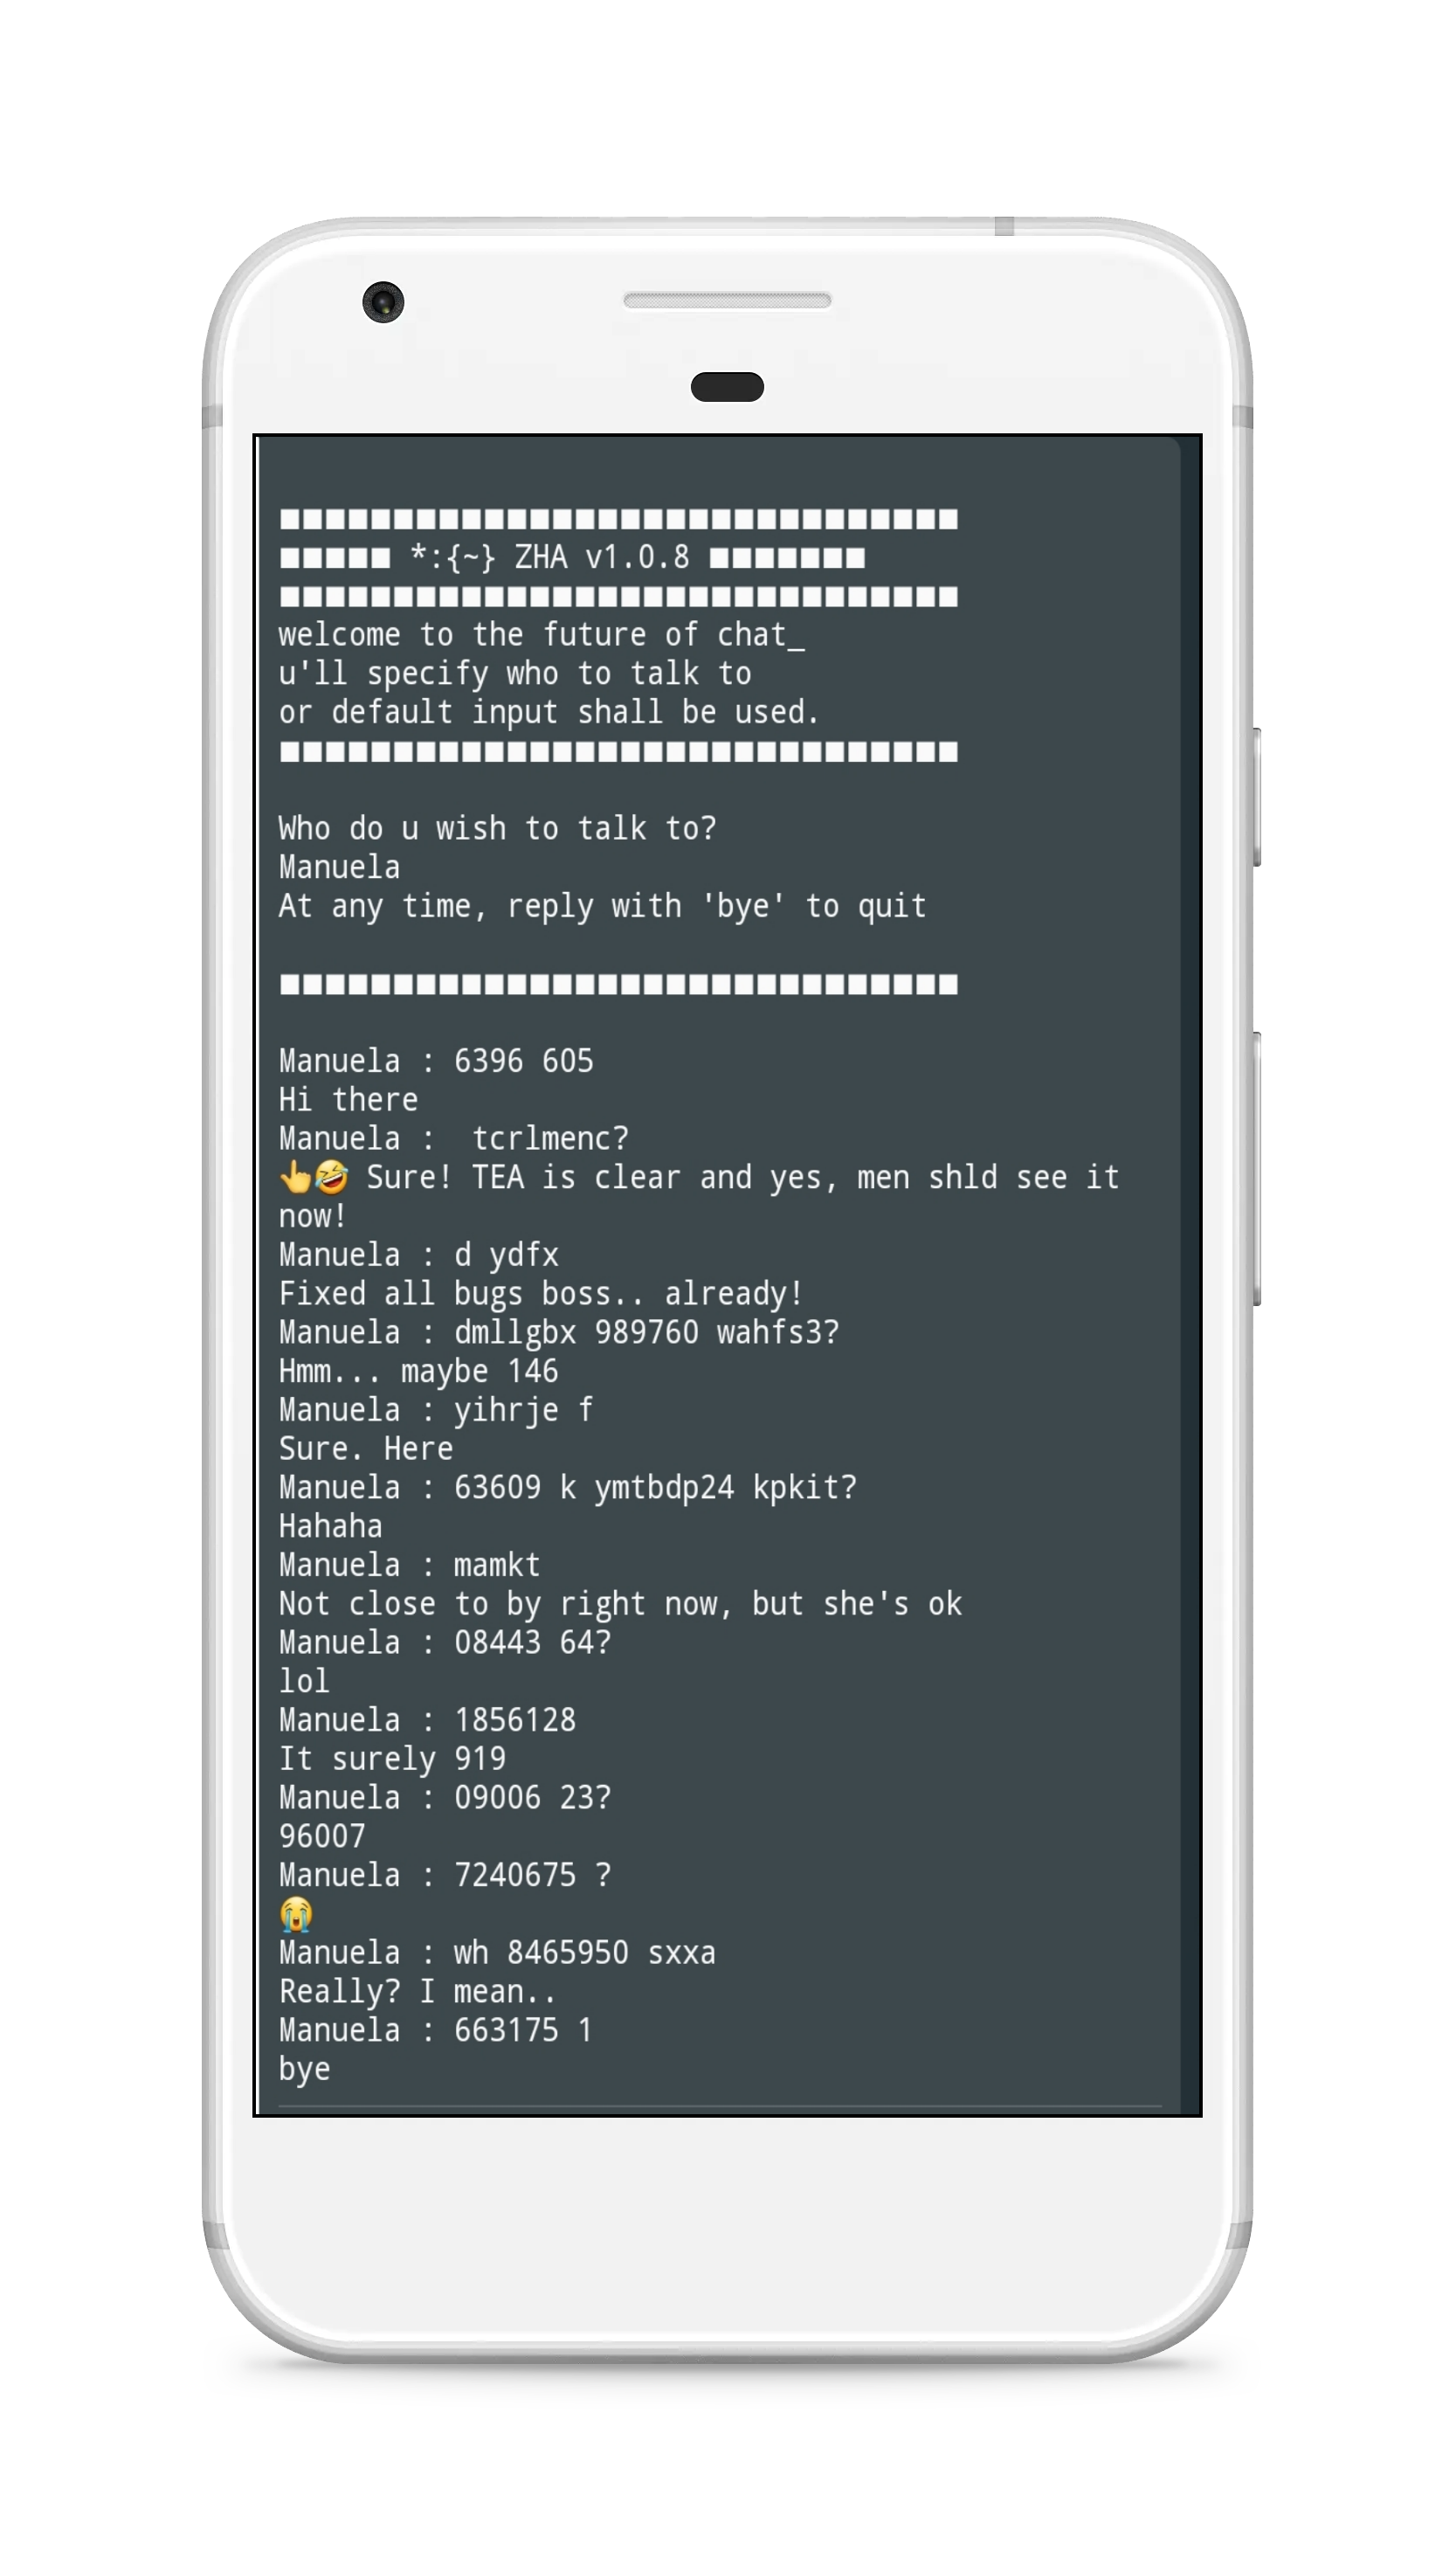
\includegraphics[width=0.4\textwidth]{resources/images/zhasession.png}\\
   \caption{A ZHA v1.0.8 session dump}
  \label{FIGZHA}
  \end{center}
\end{figure}


An example output from the latest ZHA (v1.0.8) for conversation between a fictitious character ``Manuela" and the user (lines with no leading identifying handle) is shown in \textbf{\hyperref[FIGZHA]{Figure \ref{FIGZHA}}}.



\section{Discussion}
\subsection{Strengths}
\begin{itemize}
  \item \textbf{Memorability:} 26-letter core reduces learning friction.
  \item \textbf{Compactness:} Minified programs fit in single strings, enabling embedding in constrained contexts.
  \item \textbf{Portability:} Interpreters for web and mobile enable broad deployment.
\end{itemize}

\subsection{Limitations and Risks}
\begin{itemize}
  \item \textbf{Readability:} Extreme concision can reduce readability for complex programs; tooling (formatters, debuggers) is essential.
  \item \textbf{Type and correctness:} The dynamic, transformer-based model requires careful testing and formal verification for safety-critical domains.
  \item \textbf{Ecosystem maturity:} TEA's ecosystem is nascent; adoption depends on documentation, libraries, and community tooling. However, the language has already been under-development and continuous active research since 2021, thus, it no longer is a toy nor mere academic curiosity.
\end{itemize}

\section{Related Work}

TEA intersects with minimal instruction-set languages, concatenative languages, and domain-specific text-processing languages. It draws inspiration from prior work on language design\cite{coblenz2018interdisciplinary} DSL design and the theory that many programming tasks reduce to text/sequence processing (see Lutalo, Software Language Engineering — Text Processing Language Design, 2024). Additional related projects include DNAP and other lightweight scripting languages.


TEA as a language is founded on the idea of the sequence transformer chaining paradigm, and this idea has been well formalized and developed by the same person inventing TEA, but also the new subfield of mathematics being known as 'Transformatics' \cite{Lutalo2025_transformatics_thesis}.


Coblenz et al. \cite{coblenz2018interdisciplinary} argue for integrating user‑centered design, empirical studies, and diverse evaluation methods into programming‑language design; their framework supports combining formal, performance, and human‑factors evaluations—an approach that complements TEA’s design and planned user studies.


Barash (ACM SLE '20) \cite{barash2020exampledriven} proposes an example‑driven approach to language definition and somewhat supports a commendable model for helping newbies master otherwise tricky [meta-] languages and new technologies via the concept of programming-by-example \cite{yessenov2013colorful}. The paper argues this lowers the barrier for beginner language engineers and outlines requirements for a web‑based tool supporting illustrative syntax definition. However, especially for his presentation of arguments on why many modern languages need great language support tools --- so-called language workbenches and IDEs being a core case he covered, it should be noted that research such as his did inspire good deal of the work that went into designing the reliable, portable and beginer-friendly integrated development environment for the TEA language for both mobile and web users. Also, his perspective complements TEA’s emphasis on concise, example‑rich documentation.

Concerning TEA's core focus on being a must-go-to language for arbitrary text-processing tasks, we had encountered the ideas presented in \cite{yessenov2013colorful} relating to the MIT \textbf{STEPS} project, and even though theirs attempted to provide an exhaustive solution for text-editing and processing via AI-driven coding and a meta-language, and yet, we decided to instead focus on giving the human programmer a robust language with which they can directly, and manually think-up and resolve most thorny problems related to transforming, fixing and replicating text-processing solutions in relation to working with textual data or files.

Concerning the design and language implementation choice behind keeping the TEA language an interpreted and not a compiled language, note that our familiarity with the problems surrounding attempts to bootstrap, evolve, sustain and make portable/widely-accessible, a custom or customized compiler in the modern programming landscape, as depicted in the research and reviews conducted by Huberdeau et. al (ACM SLE '24) \cite{huberdeau2024selfcompiling} in relation to their \textbf{PNUT} transpiler project was quite important. Further, we have chosen to maintain only two reference implementations of TEA (essentially, only two interpreters); one targeting the WEB environment; TEA to JavaScript; which we can likewise leverage for mobile users via methods such as exposing TEA functionality via an embedded web-browser; and the other catering for all non-web scenarios; command-line, server-side, desktop-etc via the TEA-to-Python interpreter. Somewhat similar to the intentions of PNUT, such as wanting to make C-like power available in a widely-accessible environment such as the POSIX shell, TEA was designed with the possibility of leveraging TEA programs from a POSIX shell --- such as via the \texttt{\#!/usr/bin/tttt -fc} facility --- in mind, and indeed, and rather interesting, not only can TEA programs be run from a typical POSIX shell environment (Bash and WSL being among cases we have extensively tested already), but that TEA programs can readily be embedded within existing or new POSIX shell scripts (Bash, AWK, Python, etc.).

Last but not least, experienced legacy language connoisseur and compiler engineer Vadim Zaytsev did present (ACM SLE '20) ideas on his interesting legacy-like, multiple-language inspired academic language known as \textbf{BabyCOBOL} in \cite{zaytsev2020worstnightmare}, with the intention of demonstrating many of the problematic language design quirks and aspects that make processing, but also using or evolving legacy languages somewhat undeniably tricky if not outright difficult! Interestingly, and worth noting, we did not have Zaytsev's work in mind when designing and implementing the TEA language much as most of the work occurred after the publication of his paper, and yet, later, when reviewing his findings relating to tricky features spanning legacy languages like HLASM, COBOL, REXX, PL/1 and even later ones such as SQL and AppBuilder, we did find that, even though TEA wasn't designed to be difficult to parse or process, and yet, from our experience implementing its syntax but also semantics and comparing to what he documented, that TEA's design and implementation does indeed resolve many of the tricky issues he surfaced via not actually clever, but perhaps, accidentally well-designed features of the TEA language syntax and semantics; a better use of GOTO-like control-flow, multi-level and detachable looping constructs, case-insensitive keywords, etc. 

Overall, and especially with regards to how TEA relates to, or is inspired by contemporary and earlier work in the software language engineering field (especially because, since the writing of the first language engineering review paper treating of TEA \cite{lutalo2024software} in 2024), that much of the remaining work that went into the design and implementation of the language was actually based-upon or inspired by ideas we established while reviewing ACM SLE research since the inception of the conference in 2008! However, and for purposes of keeping this manuscript brief, we shall relegate the task of a complete and paper-by-paper comparison or review, vis-a-vis what is or has been done in the TEA language project, to a future publication\footnote{A total of 32 distinctive and high-impact papers from from the ACM SLE conference have already been reviewed by the inventor of the TEA language --- see \url{https://t.me/bclectures} --- and so, it only remains to distill and compile the said review, and we hopefully shall complete in the near future.}.



\section{Conclusion and Future Work}

We presented TEA, a compact, sequence-transformer-chaining paradigm general-purpose computer programming language that is text processing oriented and which was designed with broad portability and usability in mind. TEA's minimal instruction set, bounded command space, and cross-platform interpreters make it a promising utility for low-resource programming, rapid prototyping, and domain-specific sequence analysis and transformation tasks. Future work includes:
\begin{itemize}
  \item Reviewing the language in light of the contemporary global programming language standards as well as ACM SLE-oriented cutting-edge theory and breakthroughs in language design, implementation and evaluation. 
  \item Expanding the TEA standard library (numerous currently \textit{inert} instruction signatures could find better use) based on further research into usability, feature completeness and community-feedback or demands. For example, based on ideas presented in \cite{zaytsev2020worstnightmare}, we intend to extend TEA with currently missing important facilities such as meaningful support for runtime exception handling as well as considering how to provide support for multithreaded programming. 
  \item Performance optimizations based on standardized language benchmarks, but also via rigorous industrial testing and language adaptation.
  \item User studies on learnability and productivity in low-resource environments --- especially for scenarios such as in UGANDA where the language originated and where it was initially intended to be heavily utilized.
\end{itemize}

\section*{Acknowledgments}
Thanks to the TEA project contributors and the Nuchwezi Research community for feedback and testing.

\section*{Appendix: Quick Primer on Transformatics}
\noindent Presented here based on the original 1-pager version of \cite{Lutalo2025_transformatics_thesis}, the essential foundations of the mathematics underlying TEA is as such:

\subsection{Result 1: The Empty Sequence\cite{lnspaper}}
\label{RES1}

$\Theta = \langle \rangle \implies |\Theta| = 0 \quad \land \quad \Theta \equiv \emptyset$

\subsection{Result 2: A Symbol Set\cite{Lutalo2024gtnc}}

$\psi_\beta^n = \langle \beta_{i \in [1,n]} \rangle : n \in \mathbb{N} : \invpi(\beta_i \in \psi_\beta) = 1 \quad \forall \beta_i \in \psi_\beta$

\subsection{Result 3: A Sequence\cite{lnspaper}}
\label{RES3}

$\Theta^n = \langle \theta_{i \in [1,n]} \rangle : \mathbb{N} \times \psi_\beta : n \geq 1$

\subsection{Result 4: Sequence Cardinality\cite{adtpaper}\cite{Lutalo2024gtnc}}
\label{RES4}

$\forall \Theta^n = \langle \theta_{i \in [1,n]} \rangle : \mathbb{N} \times \psi_\beta \quad \implies \quad \invpi(\Theta^n) = |\Theta^n| = n \in \mathbb{N}$ 



\subsection{Result 5: A Sequence Symbol Set\cite{ossipaper}\cite{Lutalo2024gtnc}}
\label{RES5}

$\psi(\Theta^n) = \langle \theta_{i \in [1,k]} \rangle : k,n \in \mathbb{N} \land k \geq 1 : \invpi(\theta_i \in \psi(\Theta^n)) = 1 \quad \forall \theta_i \in \Theta^n : k \leq n : \invpi(\psi(\Theta^n)) = k$


\subsection{Result 6: A Sequence Transformation\cite{transformatics}\cite{lnspaper}}

\index{transformation}\index{sequence transformation}
$\Theta^n = \langle \theta_{i \in [1,n]} \rangle : \mathbb{N} \times \psi_\beta \rightarrow \Theta^* = \langle \theta^*_{i \in [1,k]} \rangle : \mathbb{N} \times \psi_* : \psi_\beta \neq \psi_{*} \lor \psi(\Theta^n) \neq \psi(\Theta^*) \lor \overset{>}{\psi}(\Theta^n) \neq \overset{>}{\psi}(\Theta^*)$


\subsection{Result 7: A Sequence Transformer\cite{Lutalo2025transpsy}\cite{transformatics}}
\label{RES7}

$\Theta^n = \langle \theta_{i \in [1,n]} \rangle : \mathbb{N} \times \psi_\beta \xrightarrow{f(\Theta)=\Theta^*} \Theta^* = \langle \theta^*_{i \in [1,k]} \rangle: \mathbb{N} \times \psi_* 
; \quad \psi_\beta \neq \psi_{*} \lor \psi(\Theta^n) \neq \psi(\Theta^*) \lor \overset{>}{\psi_\beta} \neq \overset{>}{\psi_*}$

\subsection{Result 8: A Sequence Filter\cite{transformatics}}
\label{RES8}

$\Theta^n = \langle \theta_{i \in [1,n]} \rangle : \mathbb{N} \times \psi_\beta \xrightarrow{f(\Theta,\psi_{\beta^*})=\Theta^*} \Theta^* = \langle \theta^*_{i \in [1,k]} \rangle : \mathbb{N} \times \psi_{\beta^*} ;\\ k \in \mathbb{N} : \psi_{\beta^*} \subseteq \psi_\beta \implies \invpi(\psi_{\beta^*}) = k \leq \invpi(\psi_\beta) \implies \invpi(\Theta^*) \leq \invpi(\Theta^n) $

\subsection{Result 9: A Sequence Generator\cite{transformatics}\cite{lutalo2025transformatic}}
\label{RES9}

$\Theta^n | \emptyset \xrightarrow{f(\psi_\beta,k))=\Theta^*} \Theta^k = \langle \beta^*_{i \in [1,k]} \rangle : \mathbb{N} \times \psi_{\beta} : k \in \mathbb{N} : \forall \beta_i \in \Theta^k \implies  k \geq 1 \quad \land \quad \beta_i \in \psi_\beta = \Psi^\infty \cup \Theta^n$

\subsection{Result 10: A Sequence Sampler\cite{lutalo_2025_trans_genetics}}

$\Theta^n \xrightarrow{f(\Theta^n,k))=\Theta^k} \Theta^k = \langle \theta_{i \in [1,k]} \rangle : \mathbb{N} \times \psi(\Theta^n) : k,n \in \mathbb{N} \land k \geq 1$



\bibliographystyle{ACM-Reference-Format}
\bibliography{references}



% inner cover
% or explicitly stretch to page size
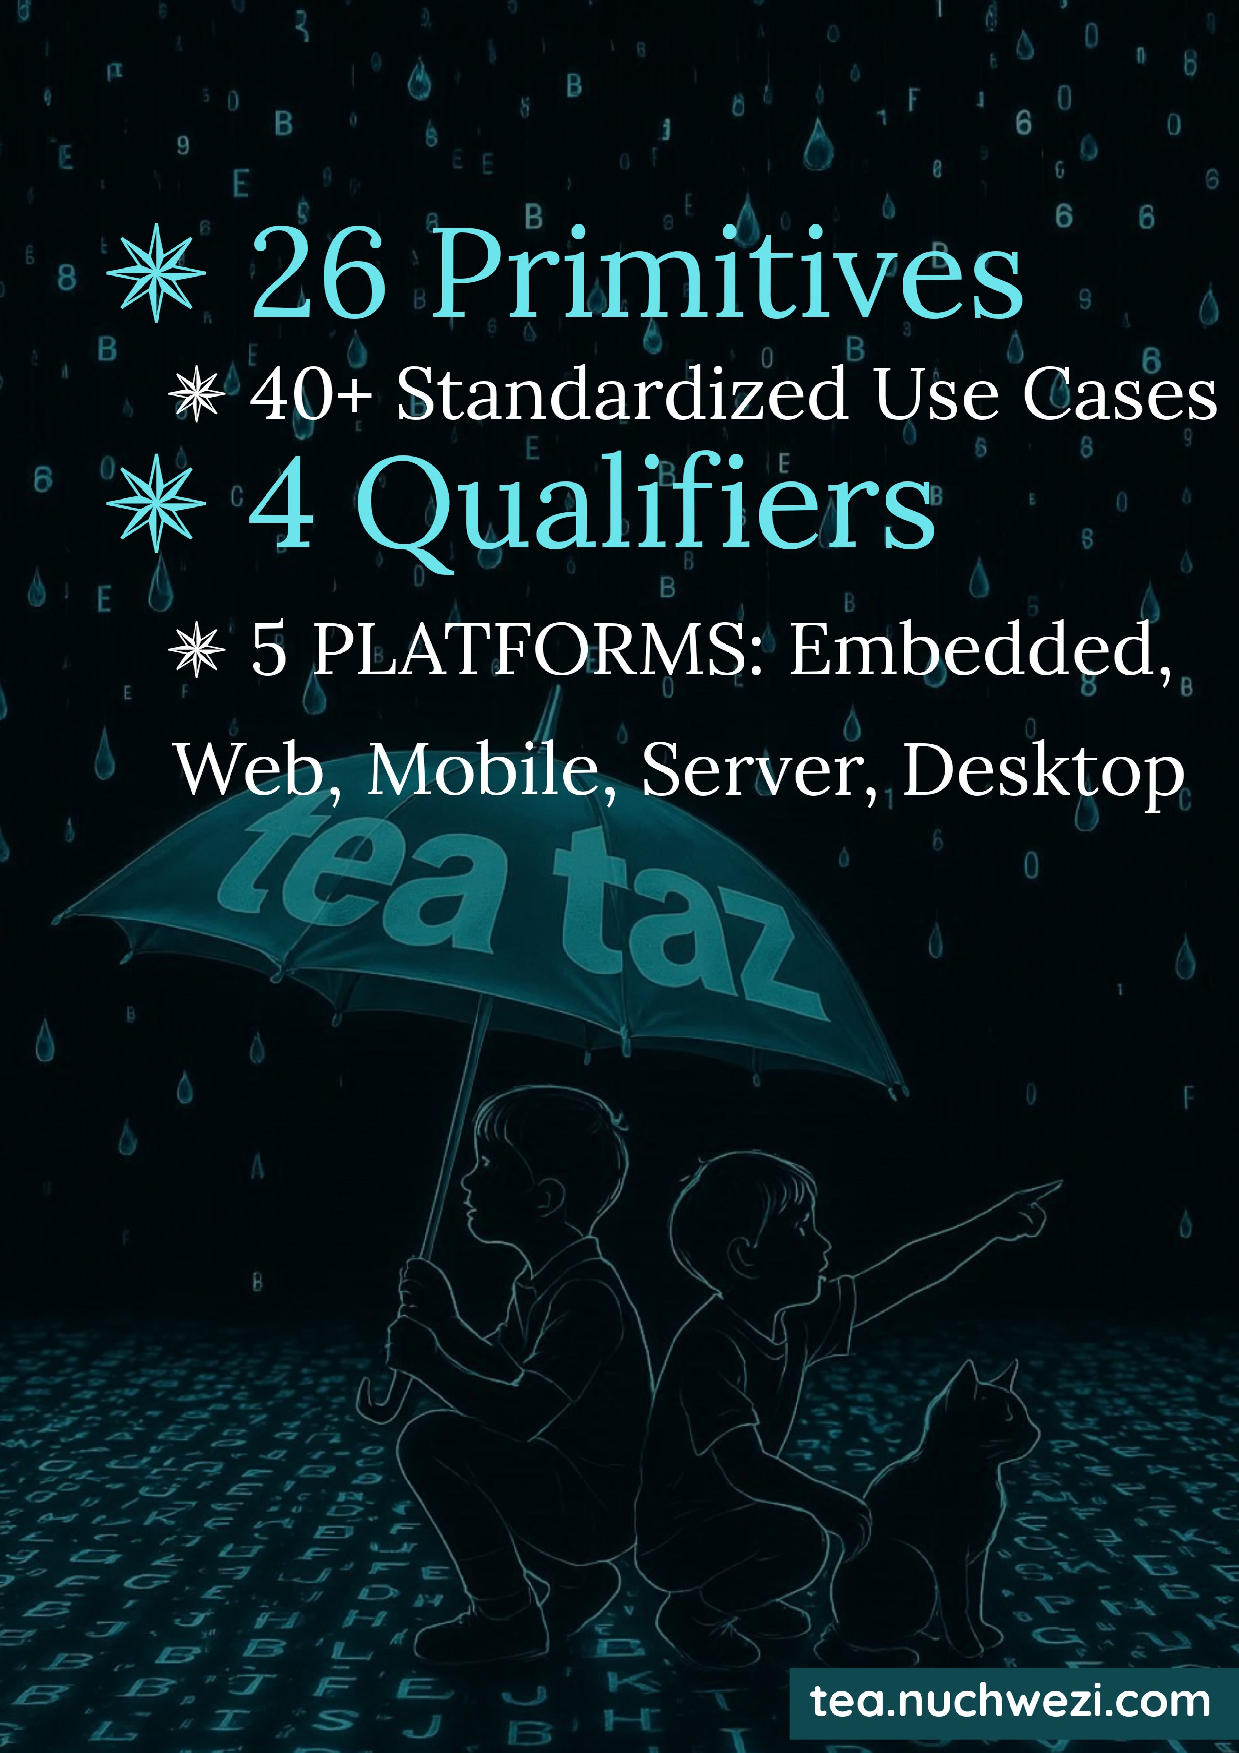
\includepdf[pages=1,
  width=\paperwidth,
  height=\paperheight,
  pagecommand={}]{resources/pdf/innercover.pdf}


% insert [back] cover --- could just be a PNG or PDF
%
\includepdf[pages=1]{resources/pdf/backcover.pdf}

% or explicitly stretch to page size

\includepdf[pages=1,
  width=\paperwidth,
  height=\paperheight,
  pagecommand={}]{resources/pdf/backcover.pdf}

\end{document}
